\subsection{Loop-Control Heterogeneity}
\label{subsec:lcu-ablation}

DISCO separates loop control from its arithmetic RCs through a per-column
Loop Control Unit (LCU). We model this distinction in OpenEdge with one LCU
per row, each using a four-register ALU and conditional branch to manage the
inner reduction loop. LCU operations issue alongside the compute PC, and a
branch is resolved at that PC boundary; the model charges one issue cycle and
checks that all row LCUs select the same target. This synchronized control is
necessary because the Python OpenEdge model has a single global PC. The output
tile loops remain statically configured, while the LCU controls the dynamic
reduction loop. The loop-counter increment and conditional branch move into
the LCU context and share PCs with the PE load and pointer-update operations;
they do not occupy standalone compute instructions. The per-row placement is
an experiment-specific organization and does not reproduce DISCO's
per-column LCU integration.

We compare the original 4$\times$4 OpenEdge mapping with two LCU-equipped
variants: 2$\times$5 (eight compute PEs and two LCUs) and 5$\times$5 (twenty
compute PEs and five LCUs). Both kernels use indirect loads and stores and
process deterministic square inputs at $N=16,32,64,128$. MMUL computes
$C=AB$; GEMM computes $C=125AB+14C$ using the original values of $C$. All 24
architecture, kernel, and size combinations match an independent CPU
reference exactly. Figure~\ref{fig:lcu-speedup} reports total simulated-cycle
speedup over the 4$\times$4 baseline, including instruction-configuration
cycles.

Neither heterogeneous mapping is faster than the original 4$\times$4
baseline in this schedule. MMUL speedups range from 0.321--0.330$\times$ for
2$\times$5 and 0.405--0.416$\times$ for 5$\times$5; GEMM ranges from
0.335--0.355$\times$ and 0.423--0.456$\times$, respectively. The 5$\times$5
variant is faster than 2$\times$5 because it has 20 rather than eight compute
PEs and therefore processes more output rows per tile. This difference cannot
be attributed to LCU count: all row LCUs execute the same loop state in
lockstep, so additional LCUs do not increase loop throughput. GEMM has a
smaller relative penalty than MMUL because its additional scaling and
read-modify-write work partly amortizes the per-tile setup.

To isolate control specialization from compute capacity, we also compare each
LCU mapping with a no-LCU reference using the same 2$\times$4 or 5$\times$4
compute mesh and the same PE instruction trace, but with the fixed-$K$ loop
fully unrolled. All matched cases are correct. PE execution cycles are
identical in each pair: the LCU does not reduce arithmetic or memory
execution time in this model. Relative to the matched reference, total-cycle
speedups range from 1.77--1.97$\times$ (MMUL) and 1.71--1.96$\times$ (GEMM)
for 2$\times$5; they range from 1.48--1.49$\times$ and 1.47--1.49$\times$,
respectively, for 5$\times$5. At $N=128$, total cycles fall by 6,219,776
(MMUL) and 6,211,584 (GEMM) in 2$\times$5, and by 2,526,784 and 2,523,456
cycles in 5$\times$5. These savings are configuration cycles from reusing
one loop body instead of configuring a copy for every reduction iteration,
not runtime branch cycles. The four local registers in each PE
are needed for the two pointers, operand/temporary, and accumulator, so a
same-capacity PE-branch implementation was not included. Per-tile pointer
initialization and the smaller compute mesh still make both LCU mappings
slower than the 16-PE 4$\times$4 baseline overall. The results are
Python-model cycle estimates, not measurements of DISCO or synthesized RTL.

\begin{figure}[t]
    \centering
    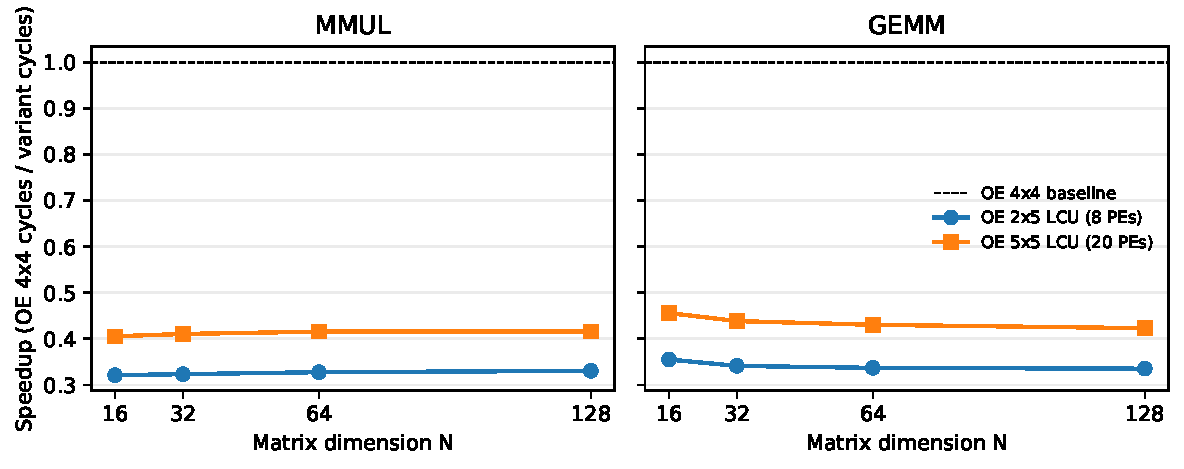
\includegraphics[width=\linewidth]{../benchmarks/DISCOvsOE/heterogeneous/heterogeneity_speedup.pdf}
    \caption{Total-cycle speedup over OpenEdge 4$\times$4 for MMUL and GEMM.
    Values below one indicate that the LCU-equipped mapping takes more cycles.}
    \label{fig:lcu-speedup}
\end{figure}
